\section{Pile-up at the LHC} \label{sec:lhc:pileup}

Given the large number of protons per bunch and the cross-section of a
proton-proton interaction, the probability to observe multiple interactions per
bunch crossing is quite high.  These multiple-interaction are known as pile-up,
$\mu$ or the time averaged representation $\langle \mu \rangle$, and come in two
different forms: 

\begin{enumerate} \item \textbf{In-time pile-up:} These are the other
proton-proton collisions that occur during the same bunch crossing as the
primary interaction that cauesd the Data Aquisition (DAQ) system to trigger.
These are the standard extra interactions we expect to observe as stated above.
\item \textbf{Out-of-time pile-up:} These are interactions that occur either
before or after a bunch crossing that causes the DAQ to trigger.  This effect is
generally due to the long integration times of some detector electronics.
\end{enumerate}

\begin{figure}[!htbp] 
  \begin{center}
    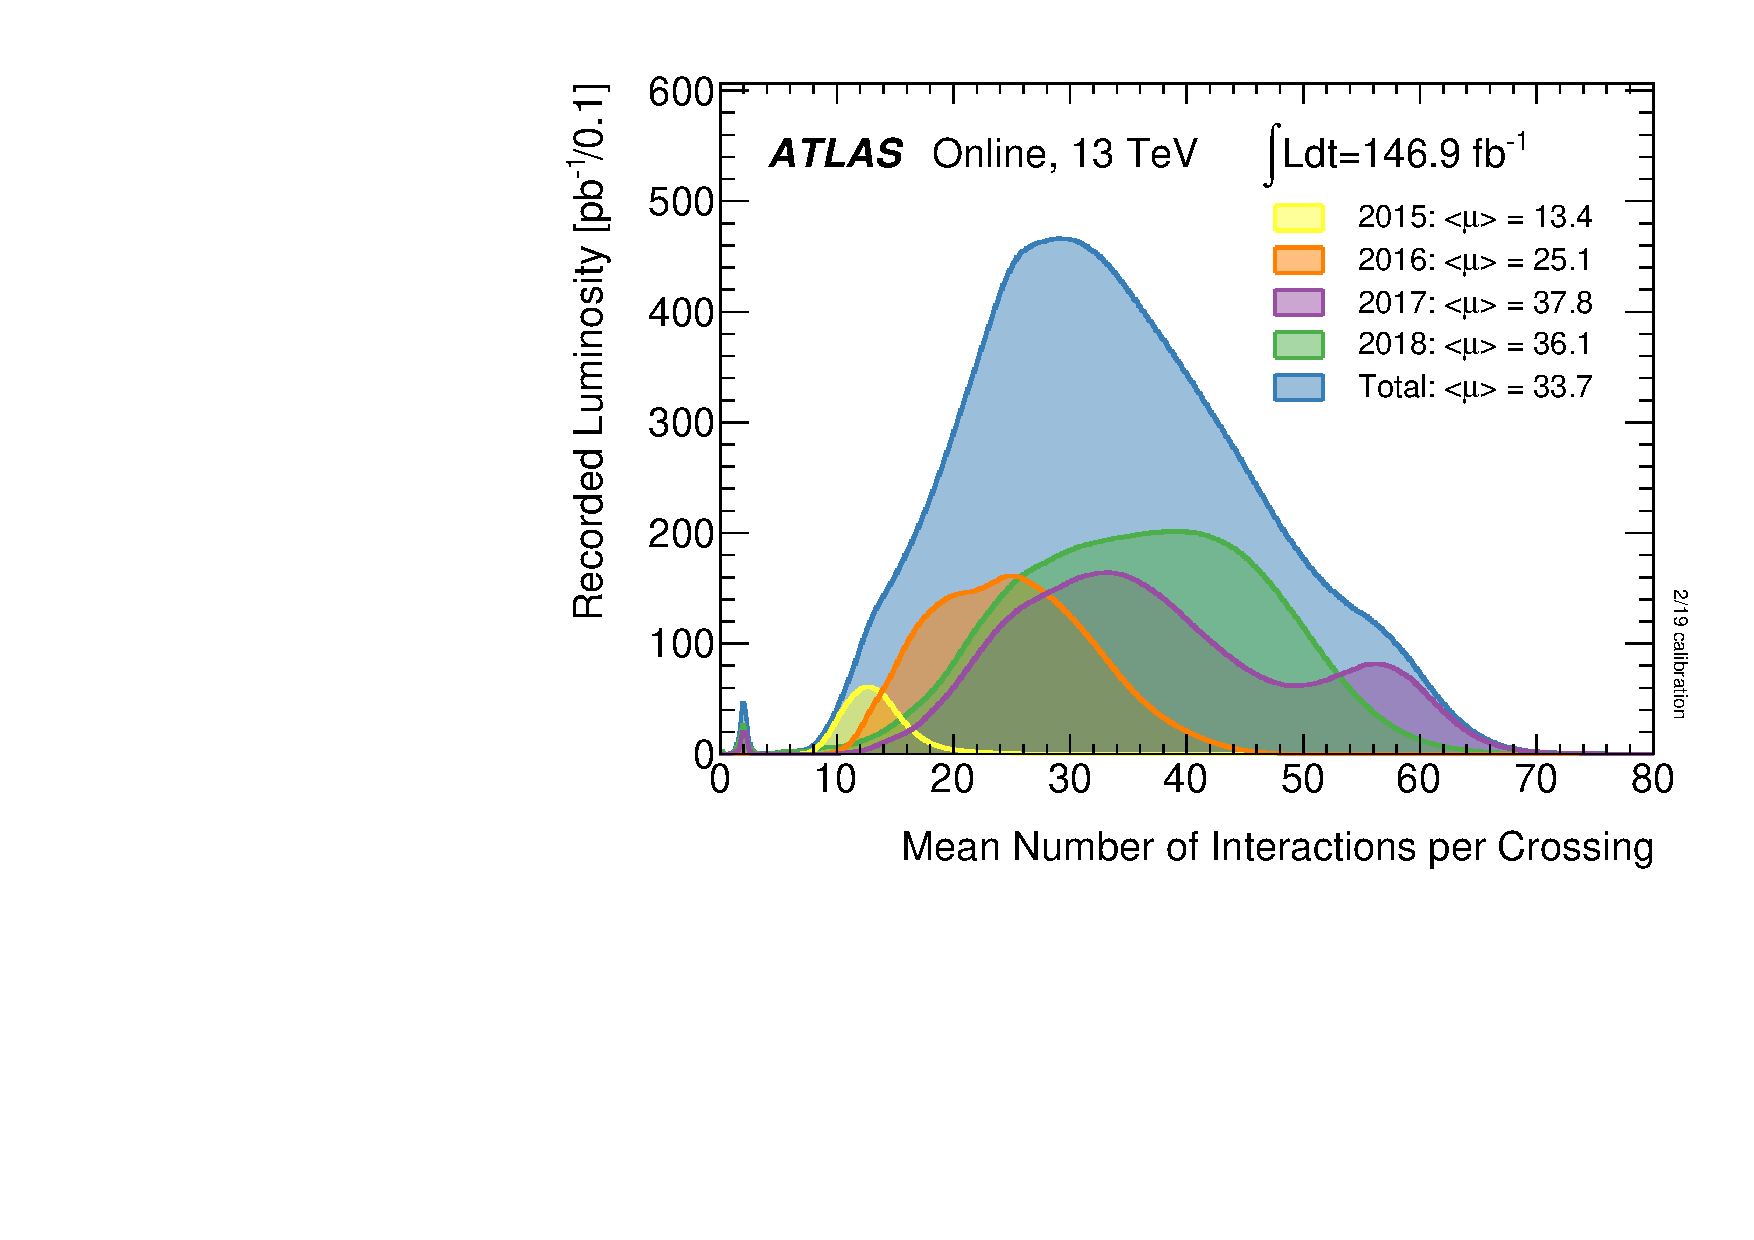
\includegraphics[width=0.9\linewidth]{figures/lhc/pileup.pdf}
    \caption{ Pileup for data taking periods 2015 - 2018} 
    \label{fig:pileup} 
  \end{center} 
\end{figure}

The pile-up profile for past years can be seen in figure \ref{fig:pileup}.  The width of this
distributino is due a combination of Poisonian statistics, the decrease in
number of protons per bunch over the lifetime of a single run, and optimization
tweaks to the beam's profile during runtime.  Understanding and eliminating the
noise from these pile-up events is crucial to reconstructing physics variables
to represent the primary interaction we hope to observe.
